\documentclass{standalone}
\usepackage{tikz}


\begin{document}
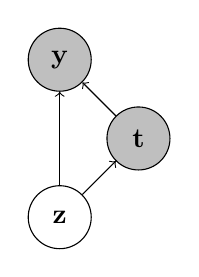
\begin{tikzpicture}
    \node[circle, draw=black, fill=lightgray, minimum size=0.8cm] (t) at (1, 1) {$\mathbf{t}$};
    \node[circle, draw=black, fill=lightgray, minimum size=0.8cm] (y) at (0, 2) {$\mathbf{y}$};
    \node[circle, draw=black, fill=white, minimum size=0.8cm] (Z) at (0, 0) {$\mathbf{z}$};
    
    \draw[->] (Z) to (t);
    \draw[->] (Z) to (y);
    \draw[->] (t) to (y);
\end{tikzpicture}
\end{document}